\chapter{IBM models}
\section{Roadmap}
The previous chapter saw the necessary background to study IBM models. This chapter consists of IBM models and their formulations. Each model consists of some assumptions and their assumptions are in the order of increasing complexity. 

The final formulation of translational model as seen in previous chapter was:
\begin{equation}
P(f\mid e) = P(m\mid e)\sum_{a}\Bigg[ \prod_{j=1}^{m}P(a_{j}\mid f_{1}^{j-1},a_{1}^{j-1},e,m)\prod_{j=1}^{m}P(f_{j}\mid f_{1}^{j-1},a_{1}^{j},e,m)\Bigg] 
\end{equation}

\section{IBM model 1}
\subsection{Formulation}
IBM model is most basic model with few assumptions which are
\begin{enumerate}
\item Length of input $m$ and output $l$ is same, i.e. $P(m \mid l) = \epsilon$

\item All alignments are equally likely, i.e. any word in the alignment $a_{j}$ can take 1 out of $(l+1)$ positions with equal probability. So
\begin{equation*}
\prod_{j=1}^{m}P(a_{j}\mid f_{1}^{j-1},a_{1}^{j-1},e,m) =
\frac{1}{(l+1)^m} 
\end{equation*}

\item Any word in the foreign sentence $f_{j}$ depends only on $j^{th}$ word in the alignment $a$ in $e$ which is $e_{aj}$. That is:\\
\begin{equation*}
\prod_{j=1}^{m}P(f_{j}\mid f_{1}^{j-1},a_{1}^{j},e,m) = \prod_{j=1}^{m}P(f_{j}\mid e_{aj})
\end{equation*}
\end{enumerate}
Considering all the three above assumptions and applying optimization steps, the IBM model-1 becomes
\begin{equation}
P(f\mid e) = \frac{\epsilon}{(l+1)^m}\prod_{j=1}^{m}\sum_{i=0}^{l}P(f_{j}\mid e_{aj})
\end{equation}


\subsection{EM for computing $P(f\mid e)$}
\subsection{Decoding in IBM model 1}
Translating a new sentence, once is model is made is called \textit{Decoding}. We apply the same Noisy-channel modal for any new sentence $f^{new}$ as

\begin{align*}
e^{best} &= argmax_{e^{new}}(P(e^{new})P(f^{new}\mid e^{new}))\\
         &= argmax_{e^{new}}\Bigg(P(e^{new})\cdot \frac{\epsilon}{(l+1)^{m}}\sum_{a}\prod_{j=1}^{m}P(f_{j}^{new}\mid e_{a_{j}}^{new})\Bigg) \\
         &= argmax_{e^{new}}\Bigg(P(e^{new})\cdot \frac{\epsilon}{(l+1)^{m}}\prod_{j=1}^{m}\sum_{i=0}^{l}P(f_{j}^{new}\mid e_{a_{j}}^{new})\Bigg) \\
         &= argmax_{e^{new}}\Bigg(\frac{\epsilon}{(l+1)^{m}}\Bigg)\cdot \big(P(e_{0}^{new}) \big)\cdot \Bigg(\prod_{i=1}^{l}P(e_{i}^{new}\mid e_{i-1}^{new})\Bigg)\cdot \Bigg(\prod_{j=1}^{m}\sum_{i=0}^{l}P(f_{j}^{new}\mid e_{a_{j}}^{new})\Bigg) \\ 
\end{align*}

IBM model is the simplest SMT model and has certain loopholes like
\begin{itemize}
\item Length of input and output are considered to be same which is very rare in real scenarios.
\item All the alignments are considered equally likely i.e. any word $e_{j}$ in $e$ can come at any position in $f$ which is again very naive.
\item For each word there is exactly 1 word associated with it. There are no null or multiple alignments.
\end{itemize}

This led to future IBM models.

\section{IBM model 2}
IBM model II has a two step process i.e. it has a lexical translation step which translates each word of the $f$ into $e$ and then the alignment step which does alignment on each word of $e$
\subsection{Formulation}
IBM model-2 takes certain assumptions into account like
\begin{enumerate}
\item Takes alignment into consideration i.e.
\begin{equation*}
\prod_{j=1}^{m}P(a_{j}\mid f_{1}^{j-1},a_{1}^{j-1},e,m) = \prod_{j=1}^{m}P(a_{j}\mid j,l,m)
\end{equation*}
\item $f_{j}$ depends on $e_{a_{j}}$ so,
\begin{equation*}
\prod_{j=1}^{m}P(f_{j}\mid f_{1}^{j-1},a_{1}^{j},e,m) = \prod_{j=1}^{m}P(f_{j}\mid e_{aj})
\end{equation*}
\end{enumerate}
So the translation model becomes,
\begin{equation}
P(f\mid e) = \epsilon\prod_{j=1}^{m}\sum_{i=0}^{l}P(i\mid j,l,m)P(f_{j}\mid e_{i})
\end{equation}

Again, IBM model II is not the best of the SMT model and has following loopholes
\begin{itemize}
\item Length of input and output are considered to be same which is too ideal.
\item No null and multiple alignments for a word, each word has exactly 1 alignment.
\end{itemize}

\section{IBM model 3}
So far IBM model didn't model number of words produced from any foreign sentence word. IBM model models this feature using fertility.

Fertility $n(\phi \mid f)$ can be defined as for each foreign word number of words $\phi = 0,1,2,\cdots$ generated. Words can be handled by considering $\phi=0$.
Also, word insertion can be modeled by considering $n(\phi \mid NULL)$.

Translation by IBM model III is a four step model which is explained by an example \ref{fig:4steps} from \cite{koehn}:
\begin{figure}[H]
        \centering
        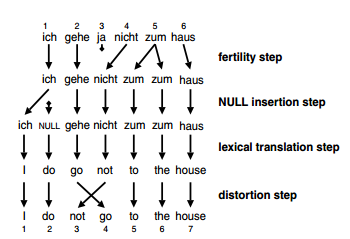
\includegraphics[scale=0.6]{Images/4steps}
        \caption{4 steps of IBM model III}
        \label{fig:4steps}
\end{figure}
\begin{enumerate}
\item Fertility Step: For each word $s_{i}$ of source sentence s, fertility $\phi_{i}$ is chosen with probability $P(\phi_{i}\mid e_{i})$.
\item Null Insertion Step: Number of target words to be generated from \textit{NULL} is chosen with probability $n(\phi \mid NULL)$.
\item Lexical Translation Step: Translation of each word similar to IBM model I is done by $P(e\mid f)$.
\item Distortion step: Probability of translating a $i_{th}$ positioned foreign word $f_{i}$ as $j_{th}$ positioned source word $s_{j}$ is modeled by $d(j\mid i,l,m)$.
\end{enumerate}

IBM model doesn't consider Alignment rather the same phenomena is captured by distortion probability. The reason being, since IBM model III introduces fertility, a single word can be broken into multiple words. Those multiple words can be rearranged into many permutations, but all those permutations will have the same alignment probability since the alignment vector for all those permutations will be entirely the same. Fig \ref{fig:distortion} explains this effect clearly,
\begin{figure}[H]
        \centering
        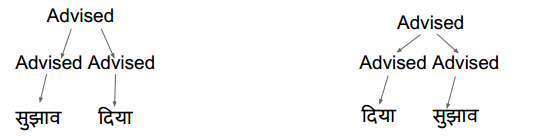
\includegraphics[scale=0.6]{Images/distortion}
        \caption{Sample example to show difference between alignment and distortion}
        \label{fig:distortion}
\end{figure}

Hence the equation for IBM model III becomes
\begin{align}
P(f\mid e) &= \sum_{a_{1}}^{l}\ldots \sum_{a_{m}}^{l}\nonumber \\
		   &= \sum_{a_{1}}^{l}\ldots \sum_{a_{m}}^{l}\binom{m-\phi_{0}}{\phi_{0}}p_{0}^{m-2\phi_{0}}p_{1}^{\phi_{0}}\prod_{i=1}^{l}\phi_{i}!n(\phi_{i}\mid e_{i})\times \prod_{j=1}^{m}t(f_{j}\mid e_{a_{j}})\mid d(j\mid a_{j},m,l)
\end{align}

IBM model III is a very strong SMT model. However, it also has certain complexity issues like
\begin{itemize}
\item When value of $m$ and $l$ are huge, the distortion matrix will be very sparse and most of the values will be zeros. It doesn't take into effect that words(phrases) that are together in the input tend to be together in the output.
\end{itemize}




















